\label{fs-framework}

Let us consider the news topic classification as an illustration of a text stream multi-classification task. There are two input streams: pre-labeled and raw. The latter stream elements must be labeled by a classifier and delivered to end-user. The pre-labeled stream is used for updating a machine learning model with new data in order to adapt it to current events. The ultimate purpose is to achieve the distribution of news topics that is changing over time. This task is a typical representative of the text stream classification problem.

Widespread classification pipeline based on bag-of-words text representation consists of three steps. The first one is computing TF-IDF features. The second one is training a classifier on these features or making a prediction. To adapt this pipeline for a stream processing engine, one needs to represent it in the form of a {\em logical graph}. It serves as a language for defining streaming computations. Vertices of a logical graph denote operations, while edges indicate data subscriptions between them. 

The initial point in our data flow is an {\em Source} vertex. It receives input texts from data producers and computes term frequencies. Computation of inverse document frequencies is a separate operation because it maintains a state and requires different data partitioning in a physical execution. {\em TF-IDF} vertex joins features corresponding to the same text and passes them to the {\em Text Classifier}. {\em Text Classifier} is the very last vertex that predicts a label and delivers it to a data consumer. The scheme of the proposed logical graph is shown in Figure~\ref{logical_graph}.

\begin{figure}[htbp]
  \centering
  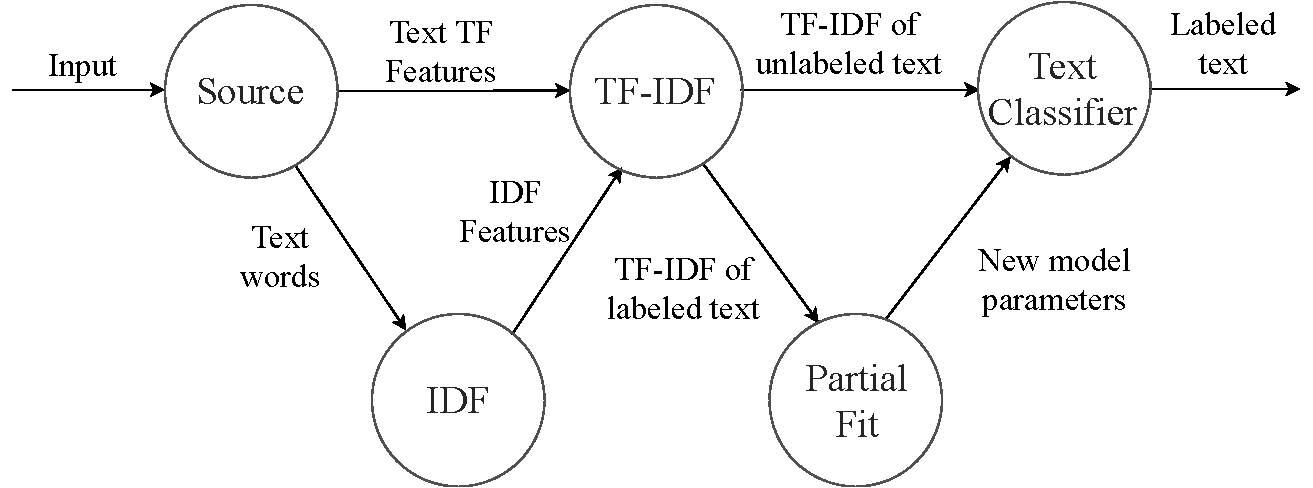
\includegraphics[scale=0.38]{pics/logical-graph}
  \caption{Text classification data flow}
  \label {logical_graph}
\end{figure}

Training pipeline is a separate branch within the logical graph introduced above. For already labeled text its features are sent to a {\em Partial fit} vertex instead of the {\em Classifier}. {\em Partial fit} vertex buffers all input elements until training is triggered. After training, the buffer flushes. Updated parameters of a machine learning model are saved for further training and broadcasted to all {\em Text Classifier} vertices.

Typical execution of this logical graph that is captured in Figure~\ref{physical_graph}. Each vertex on the scheme denotes the same computational cluster consisted of multiple units. The data partition is defined by a key, which is a word for {\em IDF} operation and text identifier for {\em TF-IDF} aggregator. Data elements with the same keys are processed on a single computational unit.

\begin{figure}[htbp]
  \centering
  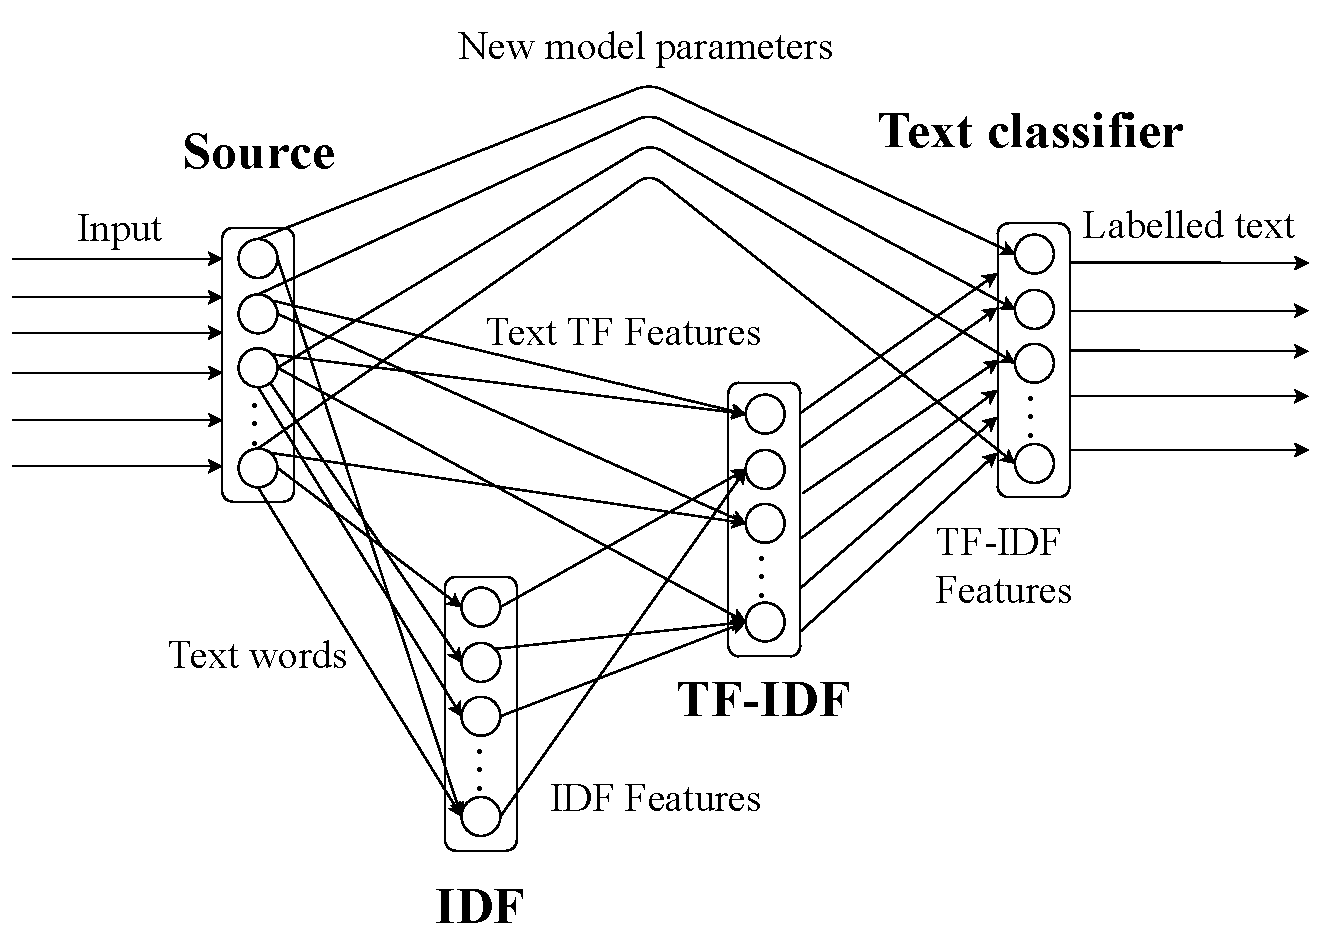
\includegraphics[scale=0.375]{pics/physical-graph}
  \caption{The physical prediction graph}
  \label {physical_graph}
\end{figure}

Despite the fact that the proposed data flow is commonly used for batch processing systems~\cite{semberecki2016distributed}, it has several potential issues regarding its execution on top of distributed stream processing engine:

\begin{itemize}
    \item There can be a race between elements before the update of {\em IDF} due to multiple asynchronous input channels as it is shown in~\ref{physical_graph}. It is unclear how such reorderings during the physical execution influence classification results.
    \item Unlike batch processing systems, streaming engines usually do not provide the same level of fault tolerance, e.g. within at least once guarantee, some input texts may be processed multiple times. Such behavior can potentially cause biased results.
    \item Training process may be time-consuming and can lead to latency spikes if training and prediction streams are not synchronized. Otherwise, it is hard to obtain reproducibility.
\end{itemize}

In the next section, we dive into details of the mentioned issues and investigate how they affect the correctness and reproducibility of classification results.